%If lack of simulation realism was one of the largest deterrents to adopting FireSim,
%modeling rationally related clocks is a stepping stone to building systems
%with dynamically scaling ones.  Useful for doing performance modeling.

Until now all Golden Gate and MIDAS-generated simulators modeled systems with a
single clock domain. Anecdotally, the lack of support for simulating targets
with more than a single clock has been the most common criticism of FireSim
offered by potential users, many of whom turn to using a conventional FPGA
prototype. The criticism is well justified: forcing the outer memory hierarchy
to run at the same frequency of the cores results in a memory hierarchy that
can sustain artificially high bandwidths at lower latencies.

To date, the only effort to validate FireSim performance against a silicon
implementation was conducted by Lee and Waterman~\cite{VLSIFireSimEval}. They
compared SPEC2006 Integer results collected from the HiFive
Unleashed~\cite{HiFiveUnleashed} against an equivalent design running on
FireSim. While the geomean of FireSim's SPEC score fell within 2\% of the
HiFive Unleashed, the largest difference was 10.7\% for \texttt{429.mcf}, a
benchmark with infamously poor memory locality (its working set has been
measured 680 MB\cite{SPEC2006WorkingSet}). The FireSim variant differed in that
it used non-standard UC Berkeley IO devices (and backing FireSim Bridges) and a
FASED memory timing model instead of their commerical DDR3/4 memory controller.
However, the most pertinent difference between the two platforms is that the
HiFive Unleashed coreplex and memory hierarchy spans three clock domains. Tiles
run at the fastest frequency~(1.5 GHz in their study), the uncore runs at half
this frequency~(75O MHz), and the DRAM memory system, capable of 2400 MT/s
(resulting in a 600 MHz controller clock in their implementation), sits in it's
own clock domain behind an asynchronous crossing\cite{FreedomU540}. To model
these domains without native support for multi-clock simulation, they resorted
to adding additional buffering between the L2 and the inner caches, and scaling
FASED latencies to match the times expected from a controller that should be
running at a slower frequency. Systems like the Freedom Unleashed, which do not actively scale frequencies
after boot, are relatively common. For these systems, support for multiple, statically defined clocks
would suffice to resolve this peformance descrepancy.

A natural place to look for inspiration is in FPGA prototyping. Here, supporting multiple clock domains is a relatively
straightforward process in theory. When mapping the ASIC design to the FPGA,
clock generating circuits, like PLLs, are replaced with FPGA
equivalents~\cite{FPMM}. While the absolute frequencies used in the prototype
will be considerably slower due to frequency limitations of the FPGA, the
relative frequencies can be maintained, and thus latencies through an SoC cache
hierarchy can be properly modeled~(the aforementioned problem of modeling
off-chip memory systems like DRAM remains).  In practise, limited availability
of clocking resources and restrictions in FPGA clock distribution can sometimes
require non-trivial changes to the ASIC RTL. To ameliorate these challenges
\emph{FPGA-Based Prototyping Methodology Manual}~\cite{FPMM} suggests a number
of Design-For-Prototyping techniques including implementing only a subset of
the clocking structures, sticking to conventional synchronous design
techniques, and isolating clock generation and distribution structures in
seperate modules at the top-level of the design hierarchy.

% DVFS stuff, prototypes
Applying the prototyping approach to a decoupled simulator---generating
multiple host-clocks whose relative frequencies match that of the target---is
an abstraction breaking change conflates host and target concerns.  In practise,
optimized models and bridges are going to be resident in different target clock
domains,and thus it will be necessary to independently gate the different
host clocks, destroying much of the merit of generating multiple clocks in
the first place. Instead, we can derive multiple simulated clocks from a single
host clock. This approach has some appealing implications:
\begin{itemize}
 \item It does not require FPGA-specific clocking resources beyond clock
 buffers capable of gating the host clock. For smaller units where the fanout
 on the clock enable is small, even these can be avoided by directly adding a clock enable
 to all state elements instead of directly gating the clock. This makes it easier
 to port the same simulator to a different FPGA.

 \item It simplies the implementation, since all simulator control logic is synchronous to 
 the same clock.
\end{itemize}

One potential benefit of generating host clocks with different frequencies is
that it has the potential to improve simulator throughput (\ref{eq:sim-perf})
by putting faster parts of the target in faster host clock domains (thus
improving the $f_{fpga}$ term). Intuitively, one would expect that a faster target clock
domain should close timing at higher frequency than a
slower one. While this is generally true, the ratio of critical-path delays
between clock domains can differ substantially from an ASIC implementation, most notably because delay through ASIC elements do
not scale uniformly across all structures when mapped to an FPGA~\cite{FPGAGap2}.
We do not rule out using multiple host clocks in the future, rather, we
argue that host clock frequencies should be selected based on simulator
critical paths specifically to improve simulator throughput, not as a means to enable
simulation of multiple clocks in the target.

Using a single host clock still enables a variety of implementation
styles. Our intial prototypes revolved around modeling clock-domain crossings
in channels. For example, one could model a two-to-one crossing from a fast clock
domain to a slow clock domain by dropping every second token or, if in the
reverse direction, duplicating every token once. An early prototype of this
approach can be found in FireSim version 1.4, which permitted users to
model a clock division in the crossing between the hub and an endpoint.
Huang et al.~\cite{centrifuge} used this to simulate targets with a DRAM memory system running
at one third the rate of the rest of the simulator. To apply this technique across
the target and not simply between bridges, we considered using Golden
Gate's hierarchy manipulations to divide the target design into synchronous
islands. Each of these islands would become seperate units transformed with an unmodified FAME transform.
In simulation mapping, Golden Gate would synthesize wire-type CDC channels between
these islands\footnote{Note that the clock-domain crossing present in target still
exists, but it is split into two synchronous halves across the models. In the future, we could
potentially pull these crossing-halves into the channel itself to improve simulation
performance.}. Clock frequency information would be baked into
these clock-crossing channels during channel synthesis. We began a prototype implementation of this
approach~(we sketched out FIRRTL transformations to perform this partitioning
and designed the channels) before reconsidering.  This approach introduced
considerable structural changes to the design's module hierarchy, making the
simulator more difficult to debug, and complicating a reimplementation of
Strober-style state snapshotting. Secondly, it introduced non-trivial
amounts of queueing when cuts between clock domains spanned large sets of signals.
Perhaps most importantly, it was considerably more complex than the solution we
ultimately selected.

% Other systems that model multiple target clocks / related work.
% DVFS stuff, prototypes

% Other approaches we considered that are LI-BDN complaint
%- Doing stuff in thechannels, and splitting the design.
%  - Diagram?
%  - Used to model memory controllers in early versions of MIDAS.
%  - Ad-hoc, difficult to validate.

\section{Implementation}
% relation to ITDC / ETDC simulators

Our approach instead was to modify the hub unit to simulate multiple clock
domains \emph{in situ}. The hub unit instantiates seperate clock buffers for
each clock domain, and selectively fires clocks and channels based on the set
of clock edges it is scheduled to simulate. A single \emph{clock bridge},
generates the clock schedule as a token stream of bit-vectors indicating which
clocks are scheduled to fire in a given simulator timestep.

\subsection{Simplifying Assumptions}


To expidite the implementation of our initial prototype, we made the following assumptions:

\begin{enumerate}
\item The behavior of all clocks can be statically deduced. To further restrict
    this, we also mandate that all clocks are in-phase and rationally related.

\item All clocks in the target must be sourced from the singleton clock bridge.
    Specifically, when in FIRRTL's low form, all clock-type members of FIRRTL
    statements and expressions must be driven by the clock bridge
    exclusively through a sequence of \texttt{Connect} statements.

\item All clock endpoints must be positive-edge triggered. Chisel has no
    native support for negative-edge-triggered or level-sensitive state elements, however, the
    user must avoid using these structures in black box verilog.

\item It must be safe to coerce asynchronous resets to synchronous ones. Unlike in 
    an ASIC implementation, the designer can exploit the fact that all clocks
    in the target will come up at time zero to avoid using asynchronous
    resets where necessary.  Our implementation still has no mechanism to
    seperately handle launching asynchronous reset edges. This restriction
    will be relaxed in Chapter~\ref{sec:dynamic-multiclock}.
\item All models and bridge must be synchronous. All bridge-bound interfaces
    must be driven and latched by state elements in the same clock domain as
        the bridge.\TODO{Think about this some more}.
\end{enumerate}

We note that all of these assumptions were implicitly made about the target in
older versions of FireSim. The only difference lies in how the target clock is
sourced: instead using an explicit bridge, the target clock was driven by a
input (this was the only legal I/O permitted on the module) on the source
FIRRTL.

Strictly speaking, a target with more than one clock cannot be an SSM, and so
generated multi-clock simulators will no longer be LI-BDNs. However, extracted
models will remain primitive LI-BDNs with reference SSMs.  We suspect that
multiclock RTL that conforms to the restrictions above can be cast as an SSM
synchronous to a single fast clock whose equivalent slow clocks have been
replaced selectively enabled state elements.

\subsection{Annotation Modifications}

Where previously all channels were implicitly synchronous to the sole target
clock, now channels bound for different units may be synchronous to different
clocks. To support this, we extended channel annotations to carry a reference
to a clock in the hub model, so that the FAME transform may associate the
correct subset of channels with each clock domain. Bridge-emitted channel
annotations indicate their clock at instantiation time,
whereas compiler-extracted models have their clock inferred (more on this
later). Additionally, we introduced a new clock-type channel
field~(\texttt{TargetClockChannel}) to label the singleton clock channel in the
simulator as this channel must be handled specially by the FAME transform and channel
synthesis.

\subsection{Modified FAME Transform}
The bulk of the complexity in supporting multiple clock domains is contained in
modified FAME transform. We show the resulting hub unit implementation in
Figure~\ref{fig:static-multiclock-wrapper}. Unlike in the single-clock
implementation, the wrapper circuit must selectively operate on a subset of
channels based which clocks are scheduled to fire.  Output state machines (shown in
blue) remain mostly unchanged but are now selectively reset based on the
scheduled clock.  We added input FSMs (shown in green), essentially a pipeline stage, to remove the fanout from
the clock token port to input channel dequeue. These too are selectively reset.

Clock scheduling is managed by a two-cycle control path (shown in orange). In
stage 1, input FSMs (in green) are reset; which allows them to dequeue an input
token in the execution of the second stage. In stage two, output FSMs are reset and a
pulse is through the target clock by enabling a dedicated clock buffer for that
domain. The pipeline advances under the largely the same firing condition as the
synchronous wrapper: all channel inputs are valid, including the clock channel, and all outputs have
enqueued or are enqueueing. Since output channels for clock domains not scheduled to fire in
stage two are not reset, their \texttt{fired} registers remain set and cannot stall the pipeline.
\TODO{handle clock token valid in diagram}

\begin{figure}
    \centering
    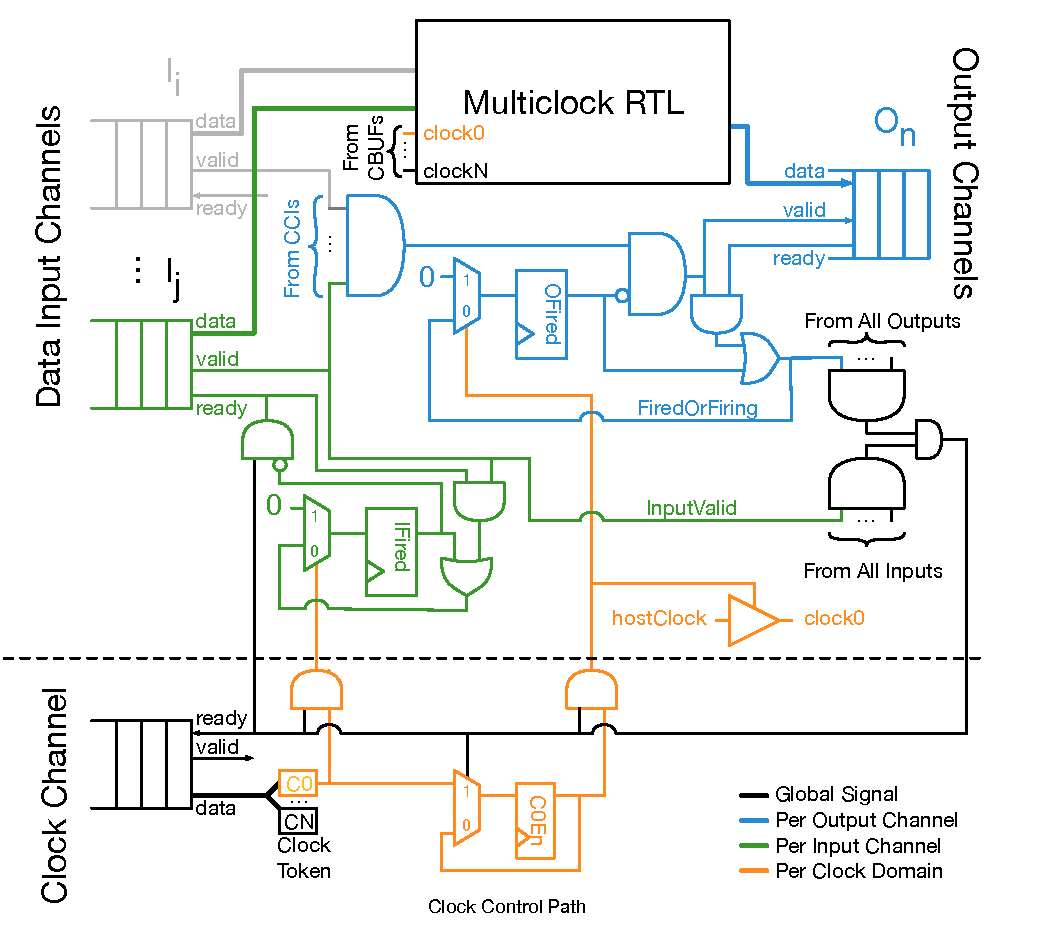
\includegraphics[width=0.99\textwidth]{figures/static-multiclock-wrapper.pdf}
    % graffle2pdf -c multiclock-wrapper midas-graphics/graffle/wrapper-transforms.graffle figures/static-multiclock-wrapper.pdf
    \caption{A wrapper-module-based conversion of multiclock target RTL with multiple clocks into a unit}
    \label{fig:static-multiclock-wrapper}
\end{figure}

\TODO{Is the extra register stage necessary?}

Initially all output FSMs are reset to zero, and the clock pipeline
register marked invalid (no clock is scheduled to fire).  This permits all combinational paths across all clock domains resolve based on the
initial input token values and target state.  As previously discussed, all
target clocks are gated under host reset such that BRAM and register state
initialized during FPGA programming cannot spuriously change as the FPGA comes
out of reset.

\subsection{Clock Bridge}

The clock bridge is responsible for determining the clock schedule by
generating an infinite token stream of $N$-wide bitvectors, where $N$ is the
number of clock domains in the target. We show an example of this encoding for three rationally
related in clock in Figure~\ref{fig:clock-token}. Each clock token corresponds to a
simulator timestep. Any clock with a positive edge in given timestep will have
its bit set in the corresponding clock token.

\begin{figure}
    \centering
    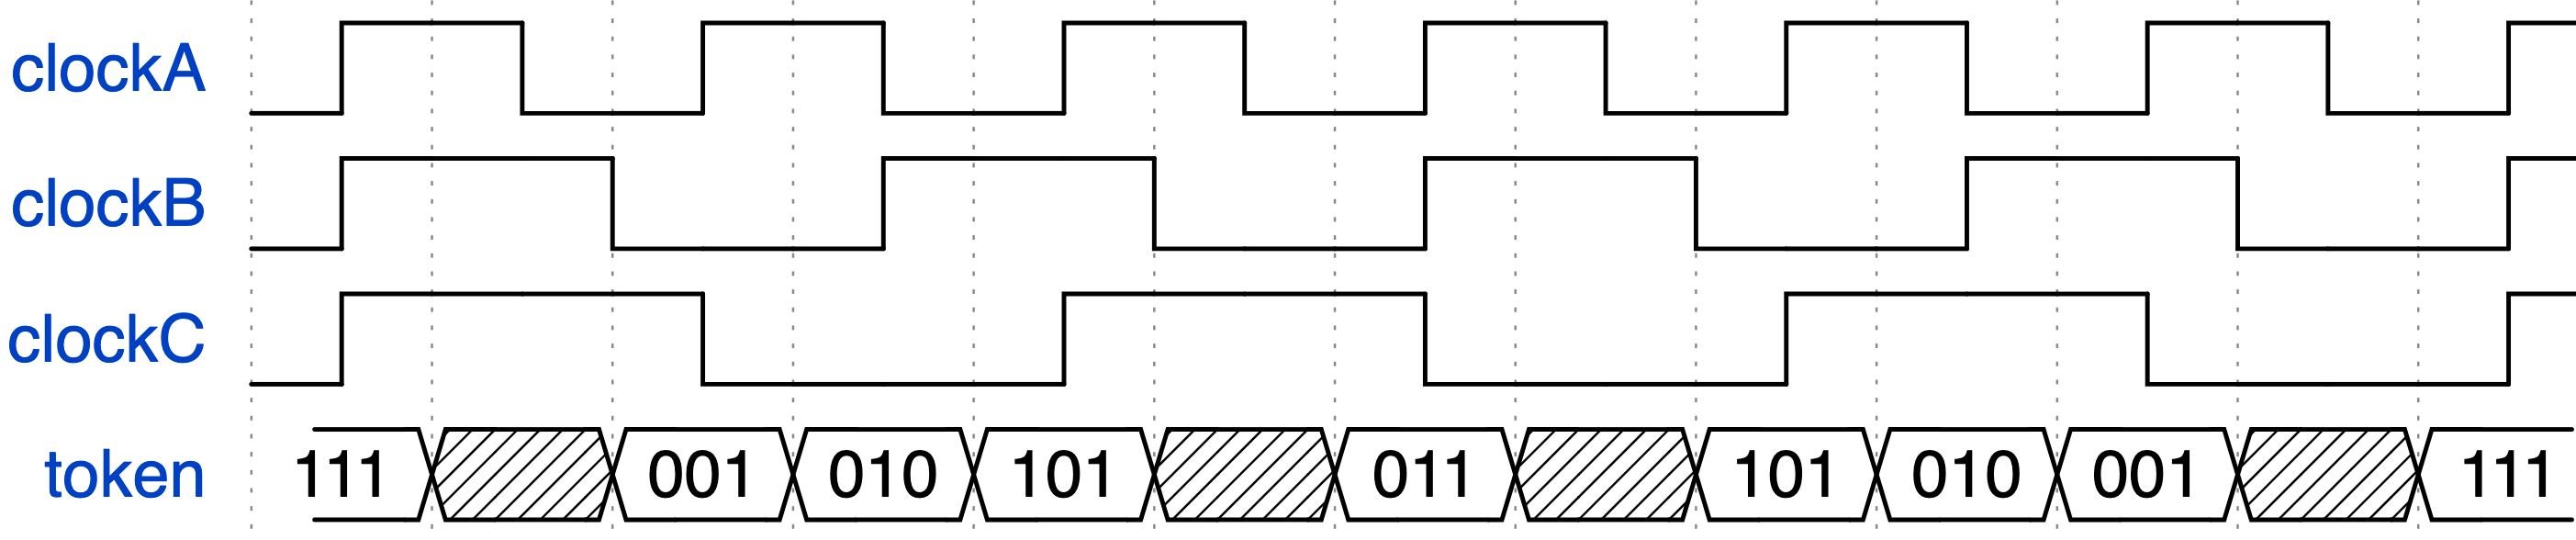
\includegraphics[width=\textwidth]{figures/clock-token.png}
    \caption{An example encoding of three rationally related clocks (clocks two and three have periods
    1.5 and 2 times longer than the first) into a clock token stream. Here there is a recurrance
    after eight tokens, with the fastest clock active in all but two tokens.}
    \label{fig:clock-token}
\end{figure}

Per our earlier assumption, the clock bridge implementation included in FireSim 1.10 accepts clock specification that
defines the frequency of all clocks as rational multiple of the
frequency of the zeroth clock\footnote{Another reasonable approach would be to
specify the periods of all clocks in an agreed upon timebase. We note
that in this case all clocks are rationally related to a fast clock whose
period equals the resolution of the timebase.}. To model a clock that is not
rationally related (e.g., a periphery clock that generated by a
secondary PLL or is sourced from off-chip), the user should select a rational
multiple that would best match the desired frequency of the clock.  During
elaboration, the clock bridge determines a virtual fast clock from which all
output clocks can be derived via an integer division (in other words, it finds
a clocks whose frequency is the least common multiple of the frequency of the
requested clocks). Then, for each output clock, it generates a series of
down-counters (\texttt{timeToNextEdge}) which are systematically reset to the
division required to generate that output clock.

To generate an output token, the bridge does the min-reduction across
\texttt{timeToNextEdge}, and broadcasts the result. All outputs whose
\texttt{timeToNextEdge} matches the minimum are scheduled clocks: their bit is
set in the output token, and their \texttt{timeToNextEdge} register is reset to
their division. Unscheduled clocks subtract the broadcasted time delta from
their registers, simulating the advance of time.  This implementation is
capable of producing a clock token with at least one bit set every host cycle.

\subsection{Other Compiler \& Bridge Modifications}

In our and our users' experience, bridges are difficult to write as they force
the developer to reason about both host and target-time considerations. To
prevent further exacerbating this problem, we elected to forbid bridges and
extracted models from having channels in multiple clock domains. This had three
primary implications:

\begin{enumerate}
\item User-instantiated bridges must explicitly indicate the clock to which
they are synchronous. Bridge-emitted channel annotations contain references to
this clock. This is a relatively trivial change, but one that affects user
facing code.

\item Debug synthesis passes must emit multiple bridges. For example, assertion
synthesis must generate a new bridge for each clock domain in which there is at
least one assertion. To do so, we built FIRRTL analyses to find source clocks
        by walking clock connectivity~(\texttt{FindClockSources}), and to group and wire
nodes (like an assertion condition) to the top-level based on each nodes source
clock(~\texttt{BridgeTopWiring}).

\item To populate channels with references to clocks in extracted models, we
introduced a transform (\texttt{FindDefaultClocks}, run before \texttt{ChannelExcision}) that analyzes top-level
clock connectivity between extracted models and the hub. Any stateful module
once extracted will have connection between a new clock output port on the hub
module and a sink port on the model (the latter port was extant prior to extraction). By
finding these connections, models can be labelled with a clock reference on the
hub model and their channels anontations can be subsequently updated.
\end{enumerate}

\subsection{The Base Clock}

In a target system with a single global clock it is natural to specify time
in cycles of that clock. Bridges can trivially track
time with a counter that tracks the number of times it has fired. Introducing
multiple clocks complicates this: specifications of time must either be made
explicit, or specified in clock cycles of some agreed-upon common clock. In
either case, these specified times cannot be compared against a bridge-local
cycle counter without the local clock's frequency, or its relative frequency to
the agreed-upon common clock. This is problematic because many of FireSim's
features use specifications of global time. For example,
instrumentation bridges (e.g., assertion and print bridges) accept
runtime arguments that specify windows of time overwhich they should be
enabled. Since these features are implemented over multiple bridges in
multi-clock targets, clock domain information must be provided to each bridge
such that they can translate time specifications into local cycle counts.

Here we exploited out assumption that all clocks are rationally related, and in
order provide a user experience similar to the existing one, we elected to
specify times in cycles of the zeroth clock generated by the bridge. We refer
to this clock as the \emph{base clock}. In Chipyard 1.4, the clock bridge is
configured to make the fastest clock in the system its base clock, which in
practise, always drives the cores of the design.

To propagate information about a bridge's clock domain to its host-side
components, we added an analysis pass, which runs during target transformation
(\texttt{TargetClockAnalysis}), that determines the clock index for each bridge
by walking clock netlist back to the clock bridge's output port. Using that
index, the pass looks up the ratio of the bridge clock relative to the base
clock. This is passed through the parameters instance to each bridge module
during platform mapping. Bridge modules typically serialize this information to the
simulation header so they can be used in the driver to recalculate times
specified in base-clock cycles in terms of their local clock.

\subsection{Rethinking Simulation Performance}

In Section~\ref{sec:iron-law}. we described simple equations that govern
simulation performance.  Under a system with multiple clocks, these need to be
updated. Amoung our users FMR~(Equation \ref{eq:fmr}) is a popular abstraction, and sees frequent use
in conversations regarding simulation performance. Perhaps, the most natural
extension of FMR for multiclock contexts is to define it in terms of the fastest
target clock:

\begin{equation}
    FMR_{fastest} = \frac{cycles_{h}}{cycles_{t,fastest}}
\end{equation}\label{eq:fmr-fastest}

Henceforth, when referring to FMR in the context of multiclock simulators we'll
be using $FMR_{fastest}$ unless otherwise stated.  Given our implementation,
when all other clocks in the target can be expressed as an integer divisions of
the fastest target clock (this target clock is the virtual fast clock), the
simulator can execute with unity FMR. This is often not the case, especially
when modeling device clocks. For example, in a two clock system where the
second clock has a frequency two thirds that of the base, the best case FMR the
simulator can achieve is $\frac{4}{3}$, since every other slow clock edge will not be
coincident with a fast clock edge and thus will require a simulator timestep in which no fast clock edge is processed.
This is reflected in the token stream illustrated in Figure~\ref{fig:clock-type}).

An alternate measure of simulator efficiency, one that reveals the presence of
host-time stalls independent of frequency selection, considers all host cycles in
which the hub model is firing at least one target clock. We define \emph{model
activity ratio}~(MAR):

\begin{equation}
    MAR = \frac{cycles_h}{timesteps}
\end{equation}\label{eq:mar}

Where \emph{timesteps} is the number of host cycles in which one or more target
clock edges are launched, or in other words, the total number of clock tokens
consumed by the hub model. Like FMR, a larger MAR corresponds to worse
simulation performance, however, in the absence of other host-time stalls all
Golden Gate simulators can run at unity MAR.

%\section{Evaluation}

% Resource utilization?
%- Clock bridge resources, fmax?
%- Scale a full system over multiple clocks

\section{Case Study - SPEC CPU 2017 Integer Performance}

Armed with the capacity to simulate multiple clock domains natively, we can
quantify the performance difference between single clock designs and more
realistic multi-clock designs. For this experiment we used otherwise standard
Chipyard designs (their block diagrams match that shown in
Figure~\ref{fig:gg-target}) and modified the clock domain organization. For
simplicity, in all cases we coupled the periphery domain to the uncore domain
denoted in Figure~\ref{fig:gg-target}. We considered three different configurations:

\begin{enumerate}
    \item A completely synchronous configuration running at 1.5 GHz. FASED DRAM timings were scaled up
        by approximately 1.5 times to match a DDR3-2133 speedgrade.
    \item A two-domain organization with the memory bus and backing DRAM subsystem sitting behind
        an asynchronous clock crossing. Here the memory bus runs at 1.0 GHz, and the rest of the system
        remains clocked at 1.5GHz.
    \item A three-domain organization that loosely matches the Freedom
        Unleashed where tiles run at 1.5 GHz and the uncore runs at 750 MHz
        with low-latency rational clock crossings between them. The DRAM memory
        system remains in an asynchronous domain running at 1 GHz.
\end{enumerate}


\begin{table}[t]
\centering
    \begin{tabular}{c c c}
    \hline
        \textbf{Parameter} & \textbf{Rocket} & \textbf{SonicBOOM} \\
    \hline
        Machine Width & 1 & 5 issue, 3 commit\\
        ROB Depth & N/A & 96 \\
        %Branch Predictor & TODO & Tage \\
        L1 I\$ Capacity & 16 KiB & 32 KiB \\
        L1 I\$ Associativity & 4-way & 8-way \\
        L1 ITLB Capacity & 32 & 32 \\
        L1 D\$ Capacity & 16 KiB & 32 KiB \\
        L1 D\$ Associativity & 4-way & 8-way \\
        L1 DTLB Capacity & 32 & 16 \\
        L1 \& L2 Block Size & \multicolumn{2}{c}{64B} \\
        L2 TLB Capacity &  \multicolumn{2}{c}{1024} \\
        L2 Cache Capacity & \multicolumn{2}{c}{2 MiB}\\
        L2 Cache Associativity & \multicolumn{2}{c}{8-way}\\
        L2 Cache Banks & \multicolumn{2}{c}{4}\\
        System Bus Width & \multicolumn{2}{c}{128b}\\
        Memory Bus Width & \multicolumn{2}{c}{256b}\\
        DRAM Speedgrade & \multicolumn{2}{c}{DDR3-2133 (14-14-14-47)} \\
        Memory Access Scheduler & \multicolumn{2}{c}{FR-FCFS} \\
    \end{tabular}
    \caption{Microarchitectural parameters of the two targets under test.}
    \label{tbl:core-parameters}
\end{table}


For each of these three organizations, we studied SoCs based around two
fundamentally different pipeline microarchitectures: Rocket~\cite{rocketchip},
a 5-stage, inorder scalar core, and SonicBOOM~\cite{SonicBOOM}, an out-of-order
superscalar core. We used the preset \texttt{Large} core configurations for
both microarchitectures; their parameters can be found
Table~\ref{tbl:core-parameters}. Since BOOM can dynamically schedule around
hazards like load misses, it should both be able to drive considerably more
memory system bandwidth (it has 4 L1 data cache MSHRs) and tolerate some
additional latency through the memory system (if it find sufficient ILP). We
kept the uncore and DRAM memory system configurations fixed across the two
designs. It was configured uses the SiFive L2 Cache Generator and a FASED-modeled,
single-channel DDR3 memory system.

\begin{figure}[htb]
    \centering
    %\captionsetup{margin=0.25cm}
    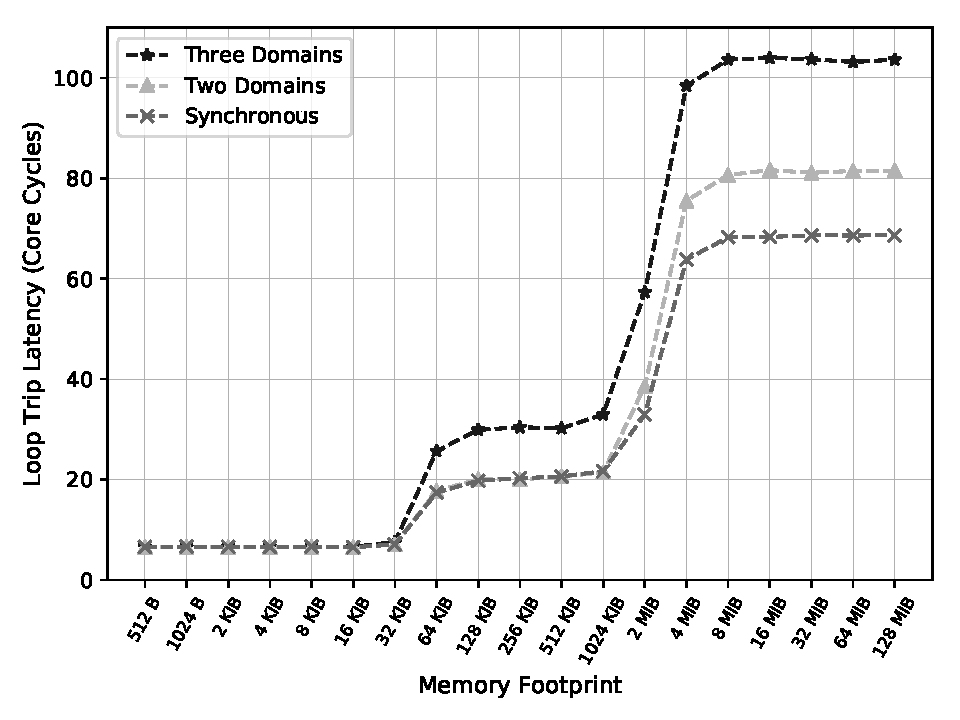
\includegraphics[width=\columnwidth]{figures/boom-ccbench.pdf}
    \caption{}
    \label{fig:boom-ccbench}
\end{figure}

We used the ccbench ``caches" micro benchmark to measure the marginal latencies
through the memory system under the three configurations. In
Figure~\ref{fig:boom-ccbench}, we show ccbench's loop trip latency when doing a
randomized pointer chase over different working set sizes (note, the pointer
chase touches each cache line only once). Marginal latency introduced the
one-domain design over the sychronous design include the asynchronous crossing
plus the additional latency intoduced by register stages now running relatively
more slowly than the cores (these could not be trivially scaled by multiplying
a configurable value). Marginal latency introduced in three domain
configuration can be attributed soley to running the uncore clock at half rate.
The rational and sychronous crossings have the same latencies, though the
rational crossing has one of it's halves running in a slower domain.

.
\begin{table}[t]
\centering
    \begin{tabular}{c@{\hskip 0.1in} S[table-format=3.2] S[table-format=3.2] S[table-format=3.2]}
    \hline
        \textbf{Benchmarks} & \textbf{Insns~(T)} &\textbf{D\$ MPKI} & \textbf{I\$ MPKI} \\
    \hline
        600.perlbench\_s & 2.98 & 9.0 & 10.0 \\
        602.gcc\_s & 2.43 & 36.6 & 9.7 \\
        605.mcf\_s & 1.60 & 97.9 & 0.1 \\
        620.omnetpp\_s & 1.11 & 56.9 & 9.3 \\
        623.xalancbmk\_s & 1.21 & 62.9 & 7.9 \\
        625.x264\_s & 4.55 & 3.0 & 2.9 \\
        631.deepsjeng\_s & 2.51 & 8.7 & 15.4 \\
        641.leela\_s & 2.59 & 5.8& 1.5 \\
        648.exchange2\_s & 3.24 & 0.0  &  0.1 \\
        657.xz\_s & 9.41 & 19.8 & 0.2 \\
    \hline
    \end{tabular}
    \caption{Dynamic instruction counts and L1 MPKIs of SPEC2017 Integer Speed (single-threaded) benchmarks.}
    \label{tbl:spec-insns}
\end{table}

To provide some insight into memory system characteristics SPEC 2017 integer
speed benchmark suite, in Table~\ref{tbl:spec-insns}, we report dynamic instruction counts,
and L1 cache misses-per-kilo-instruction (MPKIs)\footnote{These figures were
originally reported in our 2019 FASED publication.}.  We cross compiled the
benchmark suite using Speckle~\cite{Speckle} and GCC version 9.2.0 with -O2
optimizations enabled.  We ran SPEC on top of simple buildroot linux
distributions we assembled using FireMarshal~\cite{FireMarshal}.  Our
system-software setup is reproducible without modification using FireSim
version 1.11 and Chipyard 1.4, following the instructions for building SPEC2017
described in our provided documentation.

\begin{figure}[htb]
    \centering
    %\captionsetup{margin=0.25cm}
    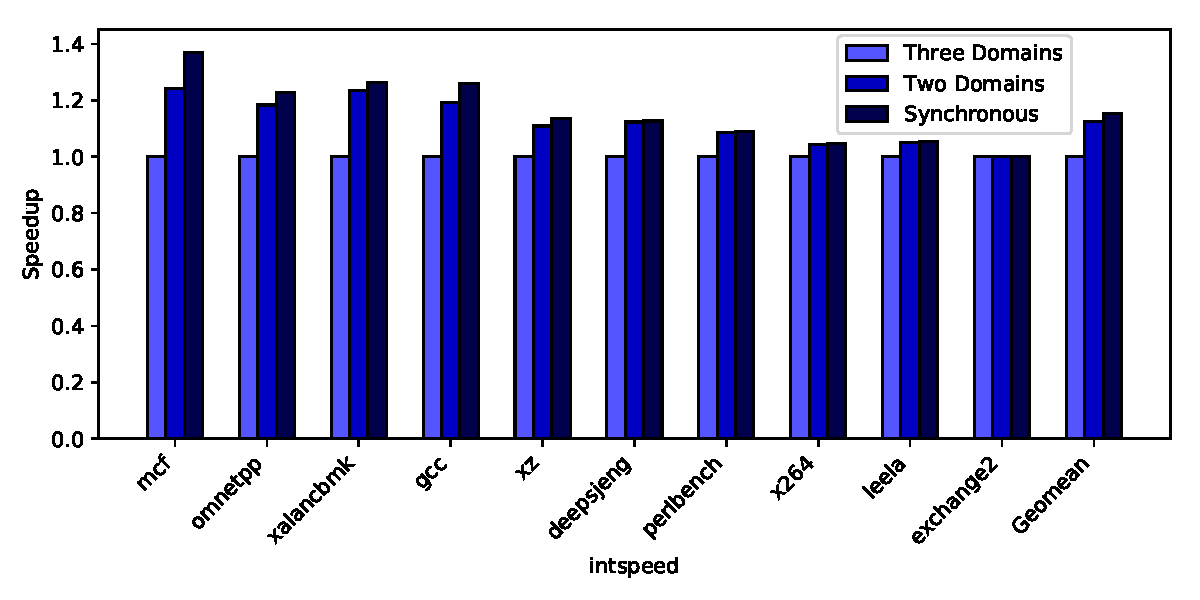
\includegraphics[width=\columnwidth]{figures/rocket-static-multiclock-speedup.pdf}
    \caption{SPEC 2017 integer speed performance on Rocket. Speedups relative to the three-domain clock organization.
    Geomean speedups for the two domain and synchronous configurations are $1.12\times$ and $1.15\times$ respectively.}


    \label{fig:rocket-static-speedup}
\end{figure}
\begin{figure}[htb]
    \centering
        %\captionsetup{margin=0.25cm}
    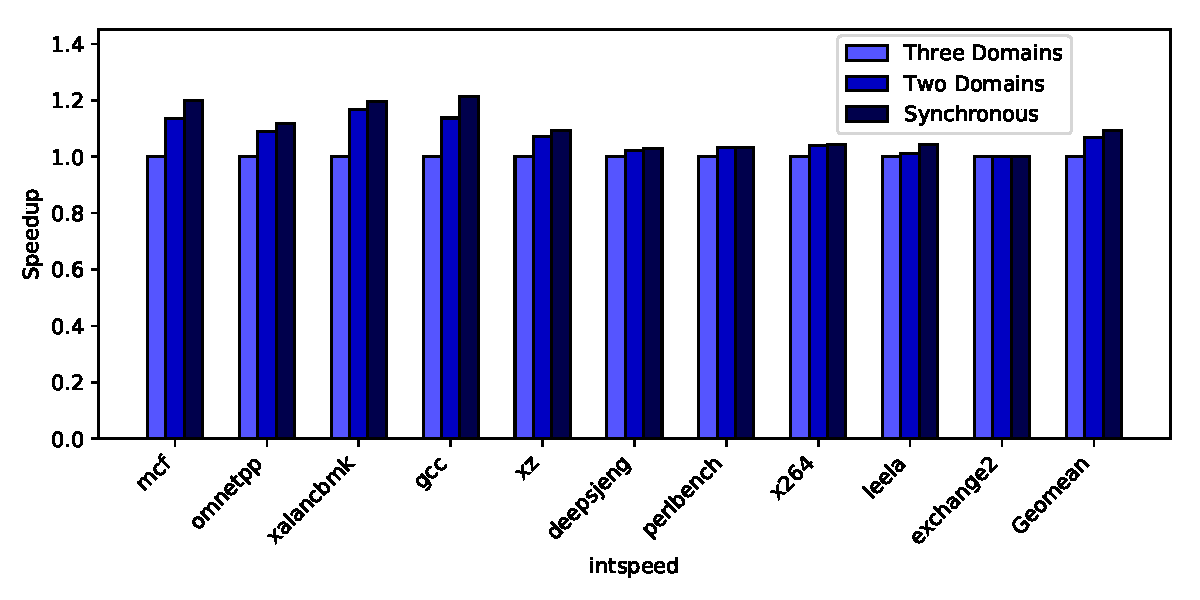
\includegraphics[width=\columnwidth]{figures/boom-static-multiclock-speedup.pdf}
    \caption{SPEC 2017 integer speed performance on BOOM. Speedups are relative to the three-domain clock organization.
    Geomean speedups for the two domain and synchronous configurations are $1.07\times$ and $1.09\times$ respectively.}
    \label{fig:boom-static-speedup}
\end{figure}


In Figures~\ref{fig:rocket-static-speedup, fig:boom-static-speedup}, we report
SPEC runtimes as speedups relative to the most detailed three-domain
configuration. BOOM designs insulated themselves better from the additional
memory system latency brought about by running the outer memory systems at
slower frequencies, with synchronous designs running $1.09\times$ faster versus
$1.15\times$ for Rocket based designs. While in Rocket's case, slow downs
correlate closely with L1 cache MPKI, BOOM's ability to dynamically schedule
around these misses complicates the story.  MCF, the benchmark with the higher
frequency of L1 Data cache misses, runs $1.37\times$ faster on a synchronous
Rocket design vs $1.20\times$ on a BOOM design. Comparably, BOOM sees its
largest performance change on 602.gcc ($1.21\times$ versus $1.26\times$ for
rocket), which reveals the core struggles to find as much ILP in that
benchmark as in other memory-intensive benchmarks, like 605.mcf.

\begin{table}[t]
\centering
    \begin{tabular}{c
        S[table-format=2.0]@{\hskip 0.30in}S[table-format=3.0]@{\hskip 0.4in}
        S[table-format=2.0]@{\hskip 0.30in}S[table-format=3.0]@{\hskip 0.4in}
        S[table-format=2.0]@{\hskip 0.30in}S[table-format=3.0]@{\hskip 0.4in}
        S[table-format=2.0]@{\hskip 0.30in}S[table-format=3.0]@{\hskip 0.4in}
        S[table-format=2.0]@{\hskip 0.30in}S[table-format=3.0]
    }
\hline
         \multirow{2}{*}{\textbf{Target}} &
         \multicolumn{2}{c}{{\hskip -0.2in}\textbf{perlbench}} &
         \multicolumn{2}{c}{{\hskip -0.2in}\textbf{gcc}} &
         \multicolumn{2}{c}{{\hskip -0.2in}\textbf{mcf}} &
         \multicolumn{2}{c}{{\hskip -0.2in}\textbf{omnetpp}} &
         \multicolumn{2}{c}{{\hskip -0.2in}\textbf{xalancbmk}} \\
        &
        \multicolumn{1}{l}{{\hskip -0.00in}time} & \multicolumn{1}{l}{{\hskip -0.05in}$f_{emul}$} &
        \multicolumn{1}{l}{{\hskip -0.08in}time} & \multicolumn{1}{l}{{\hskip -0.05in}$f_{emul}$} &
        \multicolumn{1}{l}{{\hskip -0.08in}time} & \multicolumn{1}{l}{{\hskip -0.05in}$f_{emul}$} &
        \multicolumn{1}{l}{{\hskip -0.08in}time} & \multicolumn{1}{l}{{\hskip -0.05in}$f_{emul}$} &
        \multicolumn{1}{l}{{\hskip -0.08in}time} & \multicolumn{1}{l}{{\hskip -0.00in}$f_{emul}$} \\
\hline
BOOM-1D &      19.8 &   64.5 &  21.6 &  57.0 &  22.7 &  53.1 &    11.8 &   60.3 &       8.5 &   61.9 \\
%b2d &      26.4 &   48.6 &  28.2 &  46.6 &  28.3 &  44.9 &    15.5 &   47.3 &      11.3 &   47.9 \\
BOOM-3D &      29.5 &   44.9 &  34.4 &  43.4 &  34.4 &  42.1 &    18.1 &   43.9 &      14.2 &   44.4 \\
\hline
Rocket-1D &      14.2 &  108.9 &  19.8 &  94.9 &  28.0 &  87.8 &    10.8 &  103.5 &       9.0 &  103.9 \\
%r2d &      18.9 &   82.2 &  25.8 &  77.0 &  36.4 &  74.7 &    14.3 &   80.9 &      12.0 &   80.3 \\
Rocket-3D &      20.5 &   82.2 &  30.3 &  78.0 &  44.3 &  76.2 &    16.9 &   81.2 &      14.7 &   80.8 \\
\bottomrule
\end{tabular}
\vspace{0.5cm}

%\caption{First half}
%\end{table}
%
%\begin{table}[t]
    \begin{tabular}{c
        S[table-format=2.0]@{\hskip 0.30in}S[table-format=3.0]@{\hskip 0.4in}
        S[table-format=2.0]@{\hskip 0.30in}S[table-format=3.0]@{\hskip 0.4in}
        S[table-format=2.0]@{\hskip 0.30in}S[table-format=3.0]@{\hskip 0.4in}
        S[table-format=2.0]@{\hskip 0.30in}S[table-format=3.0]@{\hskip 0.4in}
        S[table-format=2.0]@{\hskip 0.30in}S[table-format=3.0]
    }
\hline
        \multirow{2}{*}{\textbf{Target}} &
         \multicolumn{2}{c}{{\hskip -0.2in}\textbf{x264}} &
         \multicolumn{2}{c}{{\hskip -0.2in}\textbf{deepsjeng}} &
         \multicolumn{2}{c}{{\hskip -0.2in}\textbf{leela}} &
         \multicolumn{2}{c}{{\hskip -0.2in}\textbf{exchange2}} &
         \multicolumn{2}{c}{{\hskip -0.2in}\textbf{xz}} \\
        & \multicolumn{1}{l}{{\hskip -0.00in}time} & \multicolumn{1}{l}{{\hskip -0.05in}$f_{emul}$} &
        \multicolumn{1}{l}{{\hskip -0.08in}time} & \multicolumn{1}{l}{{\hskip -0.05in}$f_{emul}$} &
        \multicolumn{1}{l}{{\hskip -0.08in}time} & \multicolumn{1}{l}{{\hskip -0.05in}$f_{emul}$} &
        \multicolumn{1}{l}{{\hskip -0.08in}time} & \multicolumn{1}{l}{{\hskip -0.05in}$f_{emul}$} &
        \multicolumn{1}{l}{{\hskip -0.08in}time} & \multicolumn{1}{l}{{\hskip -0.00in}$f_{emul}$} \\
\hline
BOOM-1D &       10.0 &   63.5 &       8.5 &   62.7 &   8.9 &   64.4 &       7.1 &   65.0 &  45.3 &   62.3 \\
%b2d &       13.3 &   48.1 &      11.3 &   47.7 &  12.2 &   48.5 &       9.5 &   48.7 &  59.9 &   48.0 \\
BOOM-3D &       15.0 &   44.4 &      12.5 &   44.2 &  13.4 &   44.8 &      10.3 &   45.0 &  69.3 &   44.4 \\
\hline
Rocket-1D &       14.7 &  108.4 &      10.7 &  109.0 &   9.5 &  109.5 &       9.7 &  109.9 &  47.8 &  107.2 \\
%r2d &       19.6 &   81.8 &      14.2 &   82.2 &  12.6 &   82.3 &      12.9 &   82.5 &  63.8 &   82.1 \\
Rocket-3D &       20.4 &   81.8 &      15.9 &   82.3 &  13.3 &   82.3 &      13.0 &   82.5 &  70.7 &   82.2 \\
\bottomrule
\end{tabular}

    \caption{SPEC 2017 Integer Speed (single-threaded) emulation performance.
    We report time~(wallclock) in hours, and $f_{emul}$, the effective
    emulation frequency of the cores of the design, in MHz. Note
    that \texttt{xz} had its inputs split over two emulators to approximately
    halve its runtime.}
    \label{tbl:spec-emulation-performance}
\end{table}


\section{Scaling Target Clock Count}

For targets with relatively few clock domains, Vivado appears to be able to
successfully place and route without any additional placement constraints.
Though clock routing and distribution was significantly enchanced in Xilinx's
Ultrascale archiecture, global clock resources are still scarse to conventional
logic intconnect. Specifically, designs that require more than 24 global clock
nets be routed through the same clock region will fail in implementation.

To establish a baseline for the scalability of our approach, we attempted to synthesize a
toy target design consisting a shift register with each of its stages different
clock domain. Thus for an $N$ stage shift register, $N$ BUFGCEs will be
instantiated in the hub model. Since each stage is small, this is adversarial
design: Vivado will attempt to place all registers in the same clocking region
(to reduce path delay), only to discover it has insufficient clocking
resources to drive the sinks. We found that we could synthesize a 12-stage
pipeline before running out of global clock resources in at least one clock
region. All told, only 13 of 24 avaiable nets are used for the implementation of
the hub model: the remaining 11 are used to route clocks for IP blocks like DDR
constrollers and PCI-E, which are periodically striped down the FPGA. Excluding
the clocks used in Golden Gate-generated RTL, median global clock net
utilization across the device is 11 (ranging between 9 to 23) across the 90
available clock regions of our VU9P part.

We propose two ways to workaround this challenge. The first is obvious:
minimize the number of unique clocks required in each clock region by
preventing placement of too many unique clock loads.  This may occur naturally
if, unlike the design above, each clock domain has signifcantly more logic.
During placement, domains will tend to exclude each other as intra-domain paths
are optimized\TODO{citation}. To test this hypothesis, we synthesized a
multi-core rocket design and placed each tile in its own clock domain.
Alternatively, it may be possible to optimize the AWS shell to reduce the
number of global clock resources it requires or better isolate its clock
domains from the rest of the simulators.  In worst case, however, placement
consraints on parts of the hub unit may be required.

A second approach may be to save global clock resources by converting a gated
clock to use a clock-enable, which can be driven through logic interconnect.
This introduces a high fanout logic net, which may introduce challenges of its
own, but for relatively small clock domains could save global clock resources
by potentially reusing the ungated host clock~(if it is being routed to the
clock region already). This optimization could be implemented by Golden Gate
without user intervention.

\section{Improving Simulator Performance with Multi-Cycle Setup Constraints}

On the surface, one challenge with using a single host clock is that all timing
paths in the target must close timing at the emulator frequency.
In effect, Vivado will use the same setup relationship to close timing on paths
whose delays are many times longer than that of critical path in the fastest
clock domain. FPGA prototypes avoid this problem entirely since each
domain is driven with clocks with the same relative frequencies as would exist on the SoC, giving slower clock domains
more setup margin. When this is combined with the fact that out-of-phase
edges in slower domains can be launched between fast-clock edges, FPGA
prototypes have a considerable performance advantage over the equivalent
multi-clock FireSim emulator.

One way to close this gap is to improve host frequency by giving Vivado more
setup margin on paths in slower target clock domains. Here we exploit the
observation that, given our current clock-token generation scheme, clocks in
all but the fastest target clock domain cannot have positive edges launched in
back-to-back host clock periods. This implies that data launched in one domain
will not be captured by state elements in the same domain until at least two
host cycles later. We can indicate this to Vivado using a multi-cycle setup
constraint on all timing arcs that are internal to that domain. In many cases
this setup relationship can be larger. A clock that has a frequency $1/N$ that
of the fastest clock, can be given a setup constraint of $N$ periods.
Additionally, the presence of other clocks with frequencies that are not
integer divisions of the fastest clock, can further lengthen this constraint.
Since the clock token stream is known at compile time, Golden Gate can analyze
these relationships and emit target-specific multi-cycle constraints.  In
principle, similar constraints could be emitted for inter-clock-domain paths,
but this would require the presence of intermediate clock-tokens between the
positive edges of both domain clocks. Since this is not frequently the case,
and since there are considerably fewer timing arcs that cross clock domains, we
opted to maintain a single-cycle setup relationship on these arcs.

To illustrate the potential of these relaxations, we manually applied a
two-cycle setup constraint on all intra-domain paths in the DRAM and uncore
domains for the three-domain targets we evaluated in
Section~\ref{sec:spec-static-multiclock}. We then resynthesized both sets of
designs, with the constraints and without, with overconstrained
host-frequencies to establish an emulator $f_{max}$. We report the improved
simulator frequencies in Table~\ref{tbl:multi-cycle-constraints}. The rocket
based design saw greater improvements that BOOM likely for a few potential
reasons. Rocket tends to close timing at higher frequencies than BOOM in ASIC
processes~\TODO{check?}, delays through common structures in OoO microarchitectures scale
more poorly when mapped to FPGAs than in-order designs, and OoO cores tend to
suffer of congestion further driving up wire delay~\TODO{WongDissertation}. Taken together, the ratio
of core path-delay to uncore path-delay is closer to parity in BOOM, than in
the Rocket-based design where it is closer to the expected one-to-two ratio one
would realize in the equivalent ASIC.


\begin{table}[t]
\centering
    \begin{tabular}{c@{\hskip 0.1in} S[table-format=3.1] S[table-format=3.1] S[table-format=3.1]}
    \hline
        \textbf{Design} & \textbf{Unrelaxed $f_{max}$} & \textbf{Relaxed $f_{fmax}$} & \textbf{\% Difference} \\
    \hline
        Quad-Core Rocket & 112.5 & 168.1 & 49.4 \% \\
        Single-Core Large Boom & 70.5 & 90.0 & 28.5 \% \\
    \hline
    \end{tabular}
    \caption{Simulator $f_{max}$ for the designs of the SPEC performance
    study without (\emph{Unrelaxed}) and with~(\emph{Relaxed}) multi-cycle
    setup constraints applied.}
    \label{tbl:multi-cycle-constraints}
\end{table}


One consequence of increasing $f_{host}$ is that various extra-emulator domain
delays will now appear to have greater latency (e.g., FASED's host DRAM
requests will take more cycles to be served), which could increase FMR. To
provide some perspective on this effect, we booted linux on instances of the
relaxed and original designs that passed timing.  We report the change in
simulation performance in Table~\ref{tbl:multi-cycle-constraints-perf}. Linux
boot differs from SPEC in that has periods of sustained disk and DRAM use and
so tends to have a greater FMR. However, even in linux boot these effects only modestly reduce
the improvement brought about by the increased $f_{fpga}$.

\begin{table}[t]
\centering
    \begin{tabular}{c@{\hskip 0.4in} S[table-format=3.0] S[table-format=1.2] S[table-format=3.1]@{\hskip 0.3in}
        S[table-format=3.0] S[table-format=1.2] S[table-format=3.1]@{\hskip 0.3in} S[table-format=1.2]}
    \hline
         & \multicolumn{3}{c}{Unrelaxed} & \multicolumn{3}{c}{Relaxed} &  \\
        \textbf{Design} & $f_{fpga}$ & FMR & $f_{emul}$ & $f_{fpga}$ & FMR & $f_{emul}$ & {Speedup} \\
    \hline
        Quad-Core Rocket & 110 &  1.45 & 76.0 & 150 & 1.49 & 107.3 & {$1.41\times$} \\
        Single-Core LargeBoom & 60 & 1.57 & 38.2 & 90 & 1.65 & 54.5 & {$1.43\times$} \\
    \hline
    \end{tabular}
    \caption{Simulator $f_{max}$ for the designs of the SPEC performance
    study without (\emph{Unrelaxed}) and with~(\emph{Relaxed}) multi-cycle
    setup constraints applied.}
    \label{tbl:multi-cycle-constraints-perf}
\end{table}

\section{Future Work / Extensions}



